\section{pH-Wert}
Der pH-Wert gibt an, wie stark sauer oder basisch eine Lösung ist.
Dieser lässt sich über einen Indikator \zB Lackmus nachweisen $\rightarrow$ Säuren färben rot, Basen färben blau

\begin{center}
\begin{tikzpicture}[scale = 0.9]
  \foreach \x in {0,1,2,3,4,5,6} {
  \draw (\x,1) node {\x};
  }
  \draw (7.5,1) node {7};
  \draw[scale = 1] (7.5,0.3) node {Neutral};
  \newcounter{xtmp}
  \foreach \x in {9,10,11,12,13,14,15} {
    \setcounter{xtmp}{\x} \addtocounter{xtmp}{-1}
    \draw (\x,1) node {\arabic{xtmp}};
  }
  \draw (0.17,0.2) -- (0,0.3) -- (0.17,0.4) -- (0,0.3) -- node [scale=1,sloped,below] {Säure stärke nimmt zu} (6,0.3);
  \draw (9,0.3) -- node [scale=1,sloped,below] {Basen stärke nimmt zu} (15,0.3) -- (14.83,0.2) -- (15,0.3) -- (14.83,0.4);
\end{tikzpicture}
\end{center}

pH < 7 entspricht einer Säure. \\
pH = 7 entspricht einer neutralen Lösung. \\
pH > 7 entspricht einer Lauge.

\section{Neutralisation}
Eine Neutralisation ist eine exotherme chemische Reaktion, bei der aus einer Säurelösung und einer Baselösung Salz und Wasser entsteht.

Beispiel: \ce{HCl + NaOH <=> NaCl + H2O}

Arrhenius: \ce{H^+ + Cl^- + Na^+ + OH^- <=> Na^+ + Cl^- + H2O}

Brønsted: \ce{H3O^+ + Cl^- + Na^+ + OH^- <=> Na^+ + Cl^- + 2H2O}

\subsection{verkürzte Ionenschreibweise}
Arrhenius: \ce{H^2+ + O^- <=> H2O}

Brønsted: \ce{H3O^+ + HO^- <=> 2H2O}

\section{Flammprobe}
Bei der Flammprobe wird die Färbung der nicht leuchtenden Flamme eines Bunsenbrenners zur Identifizierung bestimmter Substanzen verwendet. Dies wird mithilfe eines Magnesiastabes durchgeführt.

\begin{center}
\begin{tabular}{|c|c|c|c|c|c|c|}
\hline \textsc{Metallion} & \ce{Li^+} & \ce{Na^+} & \ce{K^+} & \ce{Ca^2+} & \ce{Ba^2+} & \ce{Cu^2+} \\
\hline \textsc{Flammenfärbung} & rot & gelb & violett & rot - orange & grün - gelb & grün \\
\hline
\end{tabular}
\end{center}

\section{Entstehung von Säuren, Basen (Laugen) und Salzen im Überblick}
\begin{description}
   \item[Säuren:] Nichtmetalloxid + \acl{H2O} \ce{->} Säurelösung
   \begin{description}
      \item[Beispiel:] \ce{SO3 + 3H2O -> 2H3O^+ + SO4^2-}
   \end{description}
   \item[Basen (Laugen):] \begin{enumerate}
                           \item einige Metalloxide + \acl{H2O} \ce{->} Baselösung
                           \begin{description}
                              \item[Beispiel:] \ce{CaO + H2O -> Ca^2+ + 2OH^-}
                           \end{description}
                           \item unedles Metall + \acl{H2O} \ce{->} Baselösung + \acl{H2} \\
                           (K, Na, Ca)
                           \begin{description}
                              \item[Beispiel:] \ce{2Na + 2H2O -> 2Na^+ + 2OH^- + H2}
                           \end{description}
                          \end{enumerate}
   \item[Salze:] \begin{enumerate}
                  \item Baselösung + Säurelösung \ce{->} Salzlösug + \acl{H2O} (Neutralisation)
                  \begin{description}
                     \item[Beispiel:] \ce{Na^+ + OH^- + H3O^+ + Cl^- -> Na^+ + Cl^- + 2H2O}
                  \end{description}
                  \item Metalloxid + Säurelösung \ce{->} Salzlösung + \acl{H2O} \\
                  \acs{MgO}: $\mathrm{\Delta}$EN = 2,3 $\rightarrow$ Ionenverbindung! \\
                  \ce{Mg^2+ + O^2- + 2H3O^+ + SO4^2- -> Mg^2+ + SO4^2- + 3H2O}
                  \item Metall + Nichtmetall \ce{->} Salz
                  \begin{description}
                     \item[Beispiel:] \ce{Cu + Cl2 -> CuCl2}
                  \end{description}
                  \item unedles Metall + Säurelösung \ce{->} Salzlösung + \ce{H2}
                  \begin{description}
                     \item[Beispiel:] \ce{Zn + 2H3O^+ + 2Cl^- -> Zn^2+ + 2Cl^- + H2} \ifDraftQ{}
                  \end{description}
                  \item die stärkere Säure verdrängt die schwächere aus ihren Salzen
                  \begin{description}
                     \item[Beispiel:] \ce{2NaCl + 2H^+ + SO4^2- <=> Na2SO4 + 2HCl}
                  \end{description}
                 \end{enumerate}
\end{description}

\section{Säuren und Basen -- Stimmt das Gleichgewicht im Körper?}
Damit wir uns wohlfühlen, müssen sich Säuren und Basen in
 unserem Körper im Gleichgewicht befinden, ist das nicht der
 Fall, so fühlt sich der Mensch müde und abgeschlagen, leidet
 unter niedergedrückter Stimmung, hat Muskelschmerzen
 und eine spröde, schlecht durchblutete Haut. Dazu kommen
 ständige Erkrankungen wie Grippe und Erkältung und Appetitlosigkeit.
 Meist klärt erst eine Blutuntersuchung den Grund.

Der pH-Wert unseres Blutes liegt bei etwa 7,4, das heißt leicht im
 basischen (alkalischen) Bereich. Durch Stoffwechselvorgänge
 fallen ständig saure Abbauprodukte an. Um den Normalwert
 zu erhalten, werden die Säuren von basischen Verbindungen neutralisiert.
 Doch wenn Krankheiten vorliegen, zum Beispiel Stoffwechselstörungen kann das
 Gleichgewicht nicht mehr gehalten werden.
 Noch häufiger ist es, dass der Blutwert zwar noch
 im Normalbereich liegt, aber der Körper nicht mehr gegen
 die Säuren ankommt. Diese sauren Stoffwechsel-, Zwischen-
 und Endprodukte lagern sich im Bindegewebe ab. Dass sie
 entstehen können, liegt an Stress, falscher Ernährung und Bewegungsmangel.
 Maßvolle körperliche Aktivität ist wichtig,
 intensive körperliche Anstrengung jedoch kann den Säurespiegel erhöhen.

\subsection{Hilfsmittel}
Die Nahrung ist ein wesentlicher Faktor zur Erhaltung des
 Gleichgewichts von Basen und Säuren. Dabei sollte sie zu
 80\,\% aus Basen bildenden Stoffen und nur zu 20\,\% aus Säure bildenden Stoffe bestehen.
 Sicherlich können wir manches tun, indem wir die Ernährung umstellen oder anpassen.
 Darüber hinaus können sogenannte \enquote{Basenfluter} --  basische
 Mineralstoff-, Spurenelement-, Mischungen aus der Apotheke
 hier helfen. Sie enthalten \acl{20}-, \acl{19}-, \acl{11}- und
 Magnesiumsalze und wirken Infektanfälligkeiten, Verdauungsbeschwerden und Stoffwechselproblemen entgegen.

\subsection{Lebensmittel, die den Säure- und Basenhaushalt im Gleichgewicht halten}
Welche Lebensmittel machen \enquote{Sauer}, welche Basisch?
\begin{description}
   \item[Säure bildende Lebensmittel:]
   \begin{list}{}{}
      \item[Tierische Produkte:] Fleisch, Fisch, Wurst, Hühnereiweiß, Käse, Quark.
      \item[Getreideprodukte:] Teigwaren, Weißbrot, Reis, Gemüse: Rosenkohl, Spargel.
      \item[Süßigkeiten:] Zucker, Bonbons, Schokolade, Gebäck, Kuchen, Eiscreme.
      \item[Getränke:] Kaffee, Alkohol, stark kohlensäure- und phosphathaltige Getränke.
   \end{list}
\end{description}

\begin{description}
   \item[Basen bildene Lebensmitte:]
   \begin{list}{}{}
      \item[Gemüse, Salat:] Kartoffeln, Spinat, Blumenkohl, Karotten, Tomaten, Gurken, Kopfsalat.
      \item[Obst:] Apfel, Bananen, Erdbeeren, Ananas, Orangen, Pfirsich, Aprikosen, Weintrauben.
      \item[Milchprodukte:] Vollmilch, Buttermilch, Sahne, Joghurt, Kefir.
      \item[Getränke:] stille Mineralwasser, Kräutertee.
   \end{list}
\end{description}

\section{Säurehaftes, basenhaftes, salzartiges}
\begin{enumerate}
   \item In unbelebter Natur (anorganisch) \\
   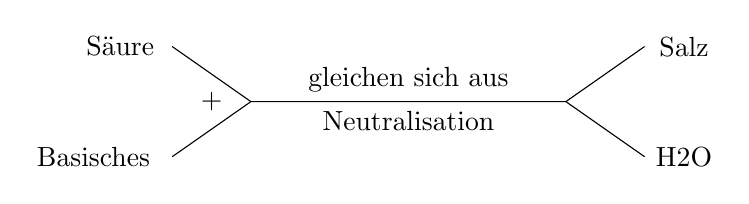
\begin{tikzpicture}
    \draw (1.34,2.7) node {Säure};
    \draw (1.0,1.3) node {Basisches};
    \draw (8.5,2.7) node {Salz};
    \draw (8.5,1.3) node {\acs{H2O}};
    \draw (2.5,2) node {+};
    \draw (2,2.7) -- (3,2) -- node [scale=1,sloped,above] {gleichen sich aus} node [scale=1,sloped,below] {Neutralisation} (7,2) -- (8,2.7);
    \draw (2,1.3) -- (3,2);
    \draw (7,2) -- (8,1.3);
   \end{tikzpicture}
   \item Betrachtung des menschlichen Körpers \\
   Das Basische ist im Innern, das Saure ist dort, wo der Mensch mit der Umgebung in Kontakt tritt.
\end{enumerate}

\section{Chemische Bindungen und Reaktionstypen -- Ein historischer Versuch}
Nachdem am 4. Juni 1783 die Brüder Montgolfier
den ersten Heißluftballon erfolgreich gestartet hatten,
sollte wenig später der Physikprofessor Charles ebenfalls einen
Ballon starten lassen.
Da er nicht wusste, welches Gas die Montgolfiers verwendet
hatten, verfiel er auf ein damals noch kaum bekanntes Gas.
Von diesem Gas waren bisher nur kleine Mengen erzeugt worden.
Charles musste deshalb zunächst eine großtechnische Apparatur erfinden:
In ein Fass wurden Eisenfeilspäne und Wasser gegeben.
Der obere Boden des Fasses hatte zwei Löcher.
Aus dem einen führte ein lederner Schlauch zum Ballon.
In das zweite, verschließbare, Loch ließ man nach und nach Schwefelsäure laufen.
Das entweichende Gas leitete man durch ein großes Gefäß mit Wasser,
um mitgerissene Schwefelsäure zu entfernen.
Die Füllung dauerte fünf Tage, dabei wurden \enquote{1000 Pfund} Eisen und
\enquote{500 Pfund} Schwefelsäure verbraucht.

\subsection{Reaktionsgleichung}
$\mathrm{\stackrel{\RM{2}}{Fe}}\;+\;$\ce{H2SO4 -> FeSO4 + H2}\\
\ce{Fe + 2H^+ + SO4^2- <=> Fe^2+ + SO4^2- + H2}

\newpage

\section{Übungen}
\subsection{\acl{NaOH} reagiert mit \acl{H2SO4}}
Arrhenius: \ce{2NaOH + H2SO4 -> Na2SO4 + 2H2O}


Brønsted: \ce{\cancel{\ce{2Na^+}} + 2OH^- + 2H^+ + \cancel{\ce{SO4^2-}} <=> \cancel{\ce{2Na^+}} + \cancel{\ce{SO4^2-}} + 2H2O}
\subsection{\acl{Ba(OH)2} reagiert mit \acl{HNO3}}
\ce{Ba(OH)2 + 2HNO3 -> Ba(NO3)2 + 2H2O}

\ce{Ba^2+ + 2OH^+ + 2H^+ + 2NO3^- <=> Ba^2+ + 2NO3^- + 2H2O}

\subsection{Bestimmen der chemischen Formel}
\begin{tabular}{ll}
\acl{Al2(SO4)3} & $\mathrm{\stackrel{\RM{3}}{Al}_2(\stackrel{\RM{2}}{SO_4})_3}$ \\
\acl{BaSO4} & \acs{BaSO4} \\
\acl{NaNO3} & \acs{NaNO3} \\
\acl{AlCl3} & \acs{AlCl3} \\
\end{tabular}

\subsection{Aufstellen von Formeln am Beispiel \aclu{Mg(OH)2}}
\begin{itemize}
   \item Feststellen der enthaltenen Ionen \ce{Mg^2+} und \ce{OH^-}
   \item (Wertigkeit \entspricht\ Ionenladung) \ac*{k.g.V.} der Wertigkeit: 2
   \item Wie oft geht die Wertigkeit ins \ac*{k.g.V.}?\\
$\mathrm{\stackrel{\RM{2}}{Mg}(\stackrel{\RM{1}}{OH})_2}$
\end{itemize}


\subsection{Schreiben Sie für folgende Reaktionen die Gleichungen}
Auch in Ionenschreibweise.

\subsubsection{\acl{MgO} reagiert mit \acl{HNO3}}
\ce{MgO + 2HNO3 -> Mg(NO3)2 + H2O} \\
$\mathrm{\Delta}$EN = 2,3 $\rightarrow$ Ionenbindung \\
A: \ce{Mg^2+ + O^2- + 2H^+ + 2NO3^- <=> Mg^2+ + 2NO3^- + H2O}
\subsubsection{\acl{13} reagiert mit \acl{H2SO4}}
\ce{2Al + 3H2SO4 -> }$\mathrm{\stackrel{\RM{3}}{Al}_2(\stackrel{\RM{2}}{SO_4})_3\,+\,}$\ce{3H2}

A: \ce{2Al + 6H^+ + 3SO4^2- <=> 2Al^3+ + 3SO4^2- + 3H2}
\subsubsection{\acl{CaCl2} reagiert mit \acl{H2SO4}}
$\mathrm{\stackrel{\RM{2}}{Ca}\stackrel{\RM{1}}{Cl}_2}$ + \ce{H2SO4 ->} $\mathrm{\stackrel{\RM{2}}{Ca}\stackrel{\RM{2}}{SO_4}}$ + \ce{2HCl}

A: \ce{Ca^2+ + 2Cl^- + 2H^+ + SO4^2- <=> Ca^2+ + SO4^2- + 2Cl^- + 2H^+}
\subsubsection{Kalziumnitrat reagiert mir \acl{Na2SO4}}
\ce{Ca(NO3)2 + Na2SO4 -> CaSO4 + 2NaNO3}

A: \ce{Ca^2+ + 2NO3^- + 2Na^+ +SO4^2- <=> CaSO4 v + 2Na^+ + 2NO3^-}
%\section{Stöchiometrie}
